\documentclass[10pt]{article}

\usepackage[letterpaper,top=0.62in,bottom=0.7in,left=0.66in,right=0.66in]{geometry}
\usepackage[T1]{fontenc}
\usepackage{lmodern}
\usepackage{microtype}
\usepackage{booktabs}
\usepackage{tabularx}
\usepackage{array}
\usepackage{graphicx}
\usepackage{xcolor}
\usepackage{placeins}
\usepackage{listings}
\usepackage{tikz}
\usetikzlibrary{arrows.meta,backgrounds,fit,positioning}
\usepackage[numbers,sort&compress]{natbib}
\usepackage[hidelinks]{hyperref}
\hypersetup{
  pdftitle={Governance Requirements for Coordinating Clinical AI Agents},
  pdfauthor={Bruce Changlong Xu, Ayush Chopra, and Alexander J. Ryu}
}

\setlength{\columnsep}{0.25in}
\setlength{\parindent}{1em}
\setlength{\parskip}{0pt}
\setlength{\emergencystretch}{2em}
\renewcommand{\familydefault}{\rmdefault}

\makeatletter
\renewcommand\section{\@startsection{section}{1}{\z@}%
  {-2.3ex \@plus -0.8ex \@minus -.2ex}%
  {0.9ex \@plus .2ex}%
  {\normalfont\sffamily\bfseries\normalsize}}
\renewcommand\subsection{\@startsection{subsection}{2}{\z@}%
  {-1.8ex \@plus -0.6ex \@minus -.2ex}%
  {0.6ex \@plus .2ex}%
  {\normalfont\sffamily\bfseries\normalsize}}
\renewcommand\subsubsection{\@startsection{subsubsection}{3}{\z@}%
  {-1.4ex \@plus -0.4ex \@minus -.2ex}%
  {0.4ex \@plus .2ex}%
  {\normalfont\sffamily\bfseries\small}}
\renewenvironment{table}[1][tbp]{\@dblfloat{table}[#1]}{\end@dblfloat}
\renewenvironment{figure}[1][tbp]{\@dblfloat{figure}[#1]}{\end@dblfloat}
\makeatother

\renewenvironment{abstract}
  {\par\small\noindent\sffamily\bfseries Abstract\enspace\normalfont\rmfamily}
  {\par}

\definecolor{circteal}{HTML}{176B87}
\definecolor{circgold}{HTML}{D99A2B}
\definecolor{circblue}{HTML}{3B6FB6}
\newcolumntype{Y}{>{\raggedright\arraybackslash}X}
\newcolumntype{B}[1]{>{\raggedright\arraybackslash\bfseries}p{#1}}
\newcolumntype{C}[1]{>{\raggedright\arraybackslash\bfseries\color{circteal}}p{#1}}
\lstdefinestyle{circjson}{
  basicstyle=\ttfamily\scriptsize,
  breaklines=true,
  columns=fullflexible,
  frame=single,
  rulecolor=\color{black!35},
  backgroundcolor=\color{black!2},
  showstringspaces=false,
  aboveskip=0.7em,
  belowskip=0.5em
}
\newcommand{\placeholderfigure}[1]{%
  \fbox{\parbox[c][1.55in][c]{0.94\linewidth}{\centering\small\color{gray}%
  Original image unavailable in supplied manuscript text.\\[0.4em]#1}}}

\title{\textbf{Governance Requirements for Coordinating Clinical AI Agents}}
\author{%
Bruce Changlong Xu$^{1}$, Ayush Chopra$^{2,3}$, Alexander J. Ryu$^{4}$\\[0.5em]
\small $^{1}$Stanford University, Palo Alto, California, USA\\
\small $^{2}$Massachusetts Institute of Technology, Cambridge, Massachusetts, USA\\
\small $^{3}$Project Iceberg at MIT, Cambridge, Massachusetts, USA\\
\small $^{4}$Mayo Clinic, Rochester, Minnesota, USA\\[0.5em]
\small Correspondence: Alexander J. Ryu, \href{mailto:Ryu.Alexander@mayo.edu}{Ryu.Alexander@mayo.edu}}
\date{}

\begin{document}

\twocolumn[
\begin{minipage}{\textwidth}
\sffamily
\noindent{\fontsize{17}{19}\selectfont\bfseries npj Digital Medicine}
\hfill{\small PERSPECTIVE}\par
\vspace{3pt}
\hrule height 1.1pt
\vspace{14pt}
{\fontsize{22}{25}\selectfont\bfseries
Governance Requirements for Coordinating Clinical AI Agents\par}
\vspace{10pt}
{\normalsize Bruce Changlong Xu$^{1}$, Ayush Chopra$^{2,3}$, Alexander J. Ryu$^{4}$\par}
\vspace{5pt}
{\footnotesize
$^{1}$Stanford University, Palo Alto, California, USA.\quad
$^{2}$Massachusetts Institute of Technology, Cambridge, Massachusetts, USA.\quad
$^{3}$Project Iceberg at MIT, Cambridge, Massachusetts, USA.\quad
$^{4}$Mayo Clinic, Rochester, Minnesota, USA.\quad
Correspondence: Alexander J. Ryu, \href{mailto:Ryu.Alexander@mayo.edu}{Ryu.Alexander@mayo.edu}.\par}
\vspace{12pt}
\rmfamily

\begin{abstract}
Clinical AI agents may create harms through interactions across shared patients, workflows, data, and
resources even when individual outputs appear acceptable. We introduce Clinical Infrastructure for
Reliable Coordination (CIRC), a conceptual framework linking a non-exhaustive taxonomy of agent-local,
interaction, and institutional risks to independent governance controls and observable evidence. CIRC
is not a standard or validated architecture; it offers a starting vocabulary for evaluating
coordination requirements before clinical deployment.
\end{abstract}
\vspace{13pt}
\hrule height 0.45pt
\vspace{14pt}
\end{minipage}
]

\section{Introduction}

Clinical artificial intelligence (AI) is shifting from decision support toward systems that choose
and execute steps in clinical or administrative workflows.\cite{moritz2025coordinated,
borkowski2025multiagent,taylor2025agents} In this Perspective, a \emph{clinical agent} pursues a
delegated objective by selecting workflow actions with less immediate human initiation than
conventional decision support. Administrative, supervised clinical, and clinically consequential
agents warrant different controls.

FHIR, SMART on FHIR, and CDS Hooks already support data exchange, authorization, and
workflow-triggered decision support.\cite{hl7fhir2019,hl7cdshooks2018,mandel2016smart} Profiles,
implementation guides, workflow engines, and local extensions can support agentic workflows. The
narrower question is which additional conventions are needed when software actors operate
continuously across organizational and vendor boundaries.

Harms can arise from stale state, unmet prerequisites, incompatible actions, retry loops, resource
congestion, or escalation without an accountable recipient. We call dependency-driven harms
\emph{interaction risks}. They do not necessarily require a new protocol: orchestration, EHR
controls, policy engines, or human-led processes may provide the needed safeguards.

Evaluation should distinguish agent-local error from failures of shared state, dependencies,
handoffs, resources, or institutional response. We introduce Clinical Infrastructure for Reliable
Coordination (CIRC) as a conceptual governance framework for requirements analysis and protocol
design, not a standard, implemented architecture, or certification scheme. CIRC contributes a
non-exhaustive risk taxonomy, independent governance levers tailored to deployment context, and a
mapping from risks and controls to observable evidence. Its trace-based example also identifies which
multi-agent risks remain untested. The levers are neither minimal nor sufficient.

\section{Existing infrastructure: capabilities and remaining gaps}

Healthcare interoperability standards already provide substantial coordination infrastructure.
FHIR Provenance and AuditEvent record actors, activities, policies, and outcomes; Task represents
work state, ownership, inputs, outputs, composite tasks, and workflow links; and Subscription supports
notifications. SMART Backend Services authorizes headless applications, while CDS Hooks invokes
services at clinical workflow events.\cite{hl7v251,hl7fhir2019,mandel2016smart,hl7cdshooks2018,
hl7smart2024}

General-purpose agent protocols add further machinery. A2A defines discovery, signed capabilities,
stateful tasks, cancellation, updates, authorization states, and extensions.\cite{googlea2a2025,
a2aspec2026} MCP connects models to isolated tool and resource servers through a host-controlled
architecture.\cite{anthropicmcp2024,mcpspec2025} ACP-style protocols support task and message
exchange.\cite{ibmacp2025} The remaining question is which healthcare-specific semantics and
conformance expectations should be shared.

Table~\ref{tab:standards} separates existing capabilities, extension or local implementation
options, and governance contracts that lack consistent standardization. Many CIRC levers can be
implemented today; CIRC links those choices to explicit risks and evidence requirements.

\begin{table}[htbp]
\centering
\caption{Existing infrastructure and the narrower coordination questions raised by CIRC.}
\label{tab:standards}
\footnotesize
\begin{tabularx}{\linewidth}{B{0.16\linewidth}YY}
\toprule
Standard or approach & Capabilities already provided & Extension or governance work for clinical-agent use \\
\midrule
FHIR resources & Structured clinical data; Task lifecycle, ownership, inputs, outputs, and composite
work; Provenance and AuditEvent; event subscriptions. & \textbf{Semantics and conformance:} profiles
can encode agent versions, dependencies, and state, but common clinical-agent profiles, required
fields, and cross-vendor behavior would need agreement. \\
SMART on FHIR & OAuth-based authorization for user-facing and headless clients; patient and encounter
context; resource-level scopes and token introspection. & \textbf{Authorization policy:} local
policy can restrict actions, but patient-specific authority, degree of autonomy, approval conditions,
and revocation across agents require explicit policy and enforcement. \\
CDS Hooks & Synchronous invocation at named clinical workflow events; context and prefetch; cards,
suggestions, and SMART app launch. & \textbf{Workflow:} useful for human-mediated checkpoints, but
not a durable multi-agent dependency graph, transaction protocol, or population resource controller. \\
A2A and ACP-style protocols & Agent discovery, capability advertisement, messages, stateful tasks,
status updates, cancellation, authentication patterns, and extensions. & \textbf{Clinical
governance:} healthcare intent, patient and encounter binding, action authority, clinical
prerequisites, accountable escalation, and safe-mode semantics require domain profiles or local rules. \\
MCP & Host-mediated access to tools, resources, and prompts; capability negotiation; isolation of
server connections; host control of permissions and consent. & \textbf{Scope:} MCP can expose
governed clinical tools, but it is not a peer-agent workflow or shared clinical dependency standard. \\
Workflow and policy engines & Stateful orchestration, business rules, human tasks, access decisions,
retries, timeouts, and compensation within a governed deployment.\cite{omgbpmn2014} & \textbf{Implementation and
portability:} these may implement CIRC levers locally; cross-vendor semantics, evidence exchange, and
institutional trust remain deployment-specific unless profiled. \\
\bottomrule
\end{tabularx}
\end{table}

The AI Risk Repository and NIST AI Risk Management Framework characterize broad AI risks and
governance functions, while clinical-agent benchmarks evaluate individual agents in realistic
environments.\cite{slattery2024risk,nist2023airmf,jiang2025medagentbench,ferber2025oncology}
Multi-agent deployment adds concurrent action on shared patients, resources, and workflows. Four
gaps illustrate the distinction.

\subsection*{Inconsistent agent observability and attribution}

FHIR Provenance and AuditEvent can distinguish human and software actors, activities, policies,
outcomes, and signatures. Consistent profiles and policies must still link each clinical action to a
stable agent and model version, delegation context, authority, and scope.

\subsection*{Unstandardized clinical intent and dependency semantics}

FHIR Task, RequestGroup, CarePlan, workflow definitions, and A2A extensions can represent clinical
dependencies. A shared profile must still specify the prerequisites, timing, state versions, resource
needs, escalation, and reversal obligations declared for each class of autonomous action.

\subsection*{Authorization without a shared model of clinical autonomy}

SMART scopes and A2A mechanisms authenticate applications, limit data access, and support additional
authorization, but their policies are implementation-specific. Deployments must define whether an
agent may read, recommend, draft, place, or execute an action; for whom and where; and with what
approval and escalation. CIRC makes these distinctions auditable rather than replacing access control.

\subsection*{Locally implemented system-level resource coordination}

Many locally reasonable agent decisions can collectively overwhelm imaging, infusion, discharge, or
specialist capacity, a pattern called a ``digital stampede.''\cite{chopra2025ripple} Standards can
represent relevant facts and workflow engines can arbitrate resources centrally, but aggregate demand
signals and population stress tests are not routinely portable across agent ecosystems.

The Ripple Effect Protocol motivates this pattern but does not validate CIRC or establish clinical
transfer. CIRC does not require its sensitivity-sharing mechanism. Any aggregate signal would need
separate evaluation for privacy, manipulation, fairness, workflow effects, and clinical safety.

\section{A non-exhaustive taxonomy of clinical-agent risk}

CIRC begins with risks rather than levels. The taxonomy is intentionally non-exhaustive: it is a
starting point for requirements analysis, not a claim to enumerate every hazard or rank deployments
on a maturity scale. We organize risks by the locus at which evidence and control are needed
(Table~\ref{tab:risk-taxonomy}). A single event can occupy more than one domain, and risk domains do
not imply causal independence.

\begin{table}[htbp]
\centering
\caption{A non-exhaustive taxonomy of clinical-agent risks.}
\label{tab:risk-taxonomy}
\small
\begin{tabularx}{\linewidth}{B{0.20\linewidth}YY}
\toprule
Risk domain & Illustrative risks & Primary unit of evaluation \\
\midrule
Agent-local evidence and reasoning & Wrong-patient or wrong-episode attribution; temporal
misalignment; substitution of codes or orders for clinical evidence; incomplete evidence retrieval;
rule misapplication; unsupported inference; false closure under missing or conflicting evidence. &
One agent's observable investigation, actions, report, and abstention behavior. \\
Interaction and workflow & Stale or inconsistent shared state; unmet prerequisites; incompatible or
duplicated actions; failed handoffs; race conditions; incorrect dependency graphs; recursive retry or
negotiation loops. & Concurrent trajectories around a shared patient, task, or care pathway. \\
System and institutional & Resource congestion; correlated failure across patients; unavailable or
misleading aggregate signals; escalation without an accountable responder; coordination-layer
outage; cross-organizational trust failure; alert burden, inequity, and drift. & Agent populations,
shared resources, institutions, and human response processes over time. \\
\bottomrule
\end{tabularx}
\end{table}

The first domain is already visible in emerging clinical-agent evaluations. CliniCARE-Bench, for
example, evaluates retrospective clinical audits over 25 scenarios and 750 patient-specific cases in
a governed, replayable EHR environment.\cite{chatrath2026clinicare} It separately scores final
verdicts, patient-evidence grounding, policy use, process adherence, and calibrated abstention. Across
16 evaluated systems, reported four-way accuracy ranged from 65.3\% to 76.1\%, while accuracy that
also excluded prohibited process shortcuts was 4.8 to 14.8 percentage points lower. Every evaluated
system over-committed more often than it over-abstained. These findings do not validate CIRC and do
not test multi-agent coordination. They demonstrate something narrower and useful: governance-relevant
properties can be specified against observable traces, and a correct output can conceal a defective
investigation.

Interaction and system risks require different evidence. A benchmark in which one agent reviews one
record cannot measure cross-agent deadlock, conflicting modifications, population-level demand, or
whether a clinician responds to an escalation. These risks require multi-agent replay, workflow stress
tests, sociotechnical simulation, prospective shadow deployment, or post-deployment monitoring. CIRC
uses the taxonomy to make those evidence boundaries explicit rather than treating single-agent
accuracy as a proxy for system safety.

\section{CIRC governance levers}

CIRC maps risks to independent governance levers (Table~\ref{tab:levers}). Each can be implemented
through a protocol, central service, EHR workflow, or another architecture at deployment-specific
strength; none is necessary, sufficient, or unique to CIRC.

The seven levers follow from questions every deployment must answer: who acted; whether the action was
permitted; what state and intent governed it; which dependencies applied; whether shared resources
were affected; who assumed responsibility; and how failure was contained. This functional
decomposition is neither empirical nor closed. Privacy, transport security, clinical validation, and
model performance remain cross-cutting obligations, and evidence may revise the set.

\begin{table}[htbp]
\centering
\caption{Lever-level crosswalk from existing infrastructure to residual coordination contracts.}
\label{tab:levers}
\footnotesize
\begin{tabularx}{\linewidth}{B{0.18\linewidth}p{0.24\linewidth}YY}
\toprule
Governance lever & Existing substrate & Residual contract and gap type & Illustrative evidence \\
\midrule
Identity and attribution & OAuth and SMART identity; A2A authentication; FHIR Provenance and
AuditEvent. & Stable agent and model version, delegation, and action linkage across systems
(semantics and conformance). & Signed identity, delegation chain, provenance, immutable audit event. \\
Scope and authorization & SMART scopes; OAuth tokens; policy engines; A2A authorization states. &
Patient-, action-, setting-, time-, and autonomy-specific authority with revocation
(authorization and governance). & Scope declaration, policy decision, override and revocation record. \\
Structured intent and shared state & FHIR Task and request resources; A2A tasks and messages; event
middleware. & Required action, patient context, state version, expiry, idempotency, and reversal
(semantics and conformance). & Typed intent, expected effect, state version, expiry, idempotency key. \\
Dependency coordination & FHIR workflow resources; BPMN and workflow engines; task cancellation. &
Cross-vendor prerequisite, acknowledgement, cancellation, and compensation behavior
(workflow and portability). & Dependency graph, release checks, acknowledgement, cancellation log. \\
Resource and population awareness & Scheduling, queueing, and capacity systems within institutions. &
Governed demand, priority, concentration, and fairness signals where needed
(implementation and governance). & Timestamped capacity and demand measures, allocation decision. \\
Operational human oversight & EHR work queues; workflow human tasks; institutional escalation policy. &
Named ownership, acknowledgement, deadline, fallback, suspension, and closure
(governance and human factors). & Assignment, response, override, fallback, and closure timestamps. \\
Monitoring and failure containment & Audit and observability platforms; rate limits; circuit breakers. &
Action-class safe modes, common-mode detection, recovery authority, and evidence
(operations and governance). & Health state, replay protection, safe-mode event, recovery log. \\
\bottomrule
\end{tabularx}
\end{table}

Profiles, extensions, workflow or policy engines, or local governance can implement these contracts
when all participants can represent, enforce, and test them. CIRC contributes the risk-to-requirement
and evidence crosswalk, not proof that a new transport is needed. Controls overlap: identity supports
audit but not state freshness; oversight contains conflict only with ownership, timing, and fallback;
and resource signals may reduce congestion while adding privacy, manipulation, and allocation risks.

\begin{figure}[htbp]
\centering
\small
\setlength{\tabcolsep}{5pt}
\begin{tabularx}{0.97\linewidth}{C{0.22\linewidth}YB{0.25\linewidth}}
\toprule
Risk locus & Governance task & Candidate levers \\
\midrule
Agent-local & Establish whether evidence, timing, policy, scope, and uncertainty support an action. &
Identity; scope; structured state; oversight \\
Interaction and workflow & Preserve shared state and dependencies as actions cross agents and
systems. & Structured intent; dependency coordination; containment \\
System and institutional & Detect correlated demand and maintain accountability during escalation
or outage. & Resource awareness; oversight; monitoring and containment \\
\bottomrule
\end{tabularx}
\caption{CIRC connects risk loci to governance tasks and candidate controls. Arrows are intentionally
not one-to-one: controls overlap, and the appropriate implementation depends on the deployment.}
\label{fig:risk-control-map}
\end{figure}

Architectures can divide levers among central workflows, policy engines, EHR services, supervisory
agents, and direct messages. Protocol fields matter most across organizational or vendor boundaries;
CIRC neither assigns every control to a new protocol nor prefers decentralized communication.

\subsection{Operational definitions and a coordination message}

An \emph{interaction risk} is a potential or realized failure attributable to interdependence among
actors, actions, shared state, or resources. A \emph{collision} occurs when actions target the same
state or resource during overlapping validity windows and violate a declared compatibility rule. A
\emph{scope violation} occurs outside authorization valid for the actor, patient, task, setting, time,
and delegated purpose. A \emph{dependency violation} releases an action despite an absent, failed,
expired, or version-incompatible prerequisite. \emph{Failure containment} holds, quarantines,
compensates, or reverses a fault before it crosses a predefined boundary.

Listing~\ref{lst:intent-message} gives a non-normative coordination message for rescheduling imaging.
Its fields could map to a FHIR profile, A2A extension, or local workflow schema; patient and encounter
references are placeholders.

\begin{lstlisting}[style=circjson,caption={Illustrative structured coordination message.},label={lst:intent-message}]
{
  "schema": "circ.intent.v0",
  "message_id": "urn:uuid:example-message",
  "idempotency_key": "schedule-change-example-1",
  "actor": {
    "agent_id": "agent:scheduling:example",
    "version": "3.2.1",
    "issuer": "Organization/institution-a"
  },
  "authority": {
    "action": "schedule.modify",
    "delegated_by": "PractitionerRole/care-team",
    "policy": "Policy/outpatient-scheduling-v4"
  },
  "subject": {
    "patient": "Patient/example",
    "encounter": "Encounter/example"
  },
  "state": {
    "version": "W/example-etag",
    "observed_at": "2030-01-15T14:30:00Z"
  },
  "intent": {
    "proposed_action": "reschedule imaging",
    "target": "Task/imaging-example",
    "reason": "capacity adjustment"
  },
  "dependencies": [
    {"task": "Task/oncology-clearance", "required_state": "completed"},
    {"task": "Task/observation-visit", "constraint": "must_remain_scheduled"}
  ],
  "valid_until": "2030-01-15T15:00:00Z",
  "reversal": {"action": "restore_prior_slot", "deadline_minutes": 30},
  "escalation": {
    "owner_role": "oncology attending",
    "respond_by": "2030-01-15T14:50:00Z",
    "on_timeout": "hold"
  },
  "signature": "detached-jws:example"
}
\end{lstlisting}

The message exposes enough context to authenticate the actor, evaluate authority, compare state,
inspect prerequisites, deduplicate retries, enforce expiry, and route conflict. Message validity does
not imply clinical validity; it makes decision context inspectable and enforceable.

\subsection{One possible deployment architecture}

Figure~\ref{fig:architecture} shows one centralized realization. A coordination service or workflow
engine checks identity and policy, binds actions to EHR state, records audit evidence, and routes
named human escalation. External agents remain subject to local policy. Equivalent controls may be
distributed, embedded in the EHR, or divided among existing services.

\begin{figure}[htbp]
\centering
\resizebox{0.98\linewidth}{!}{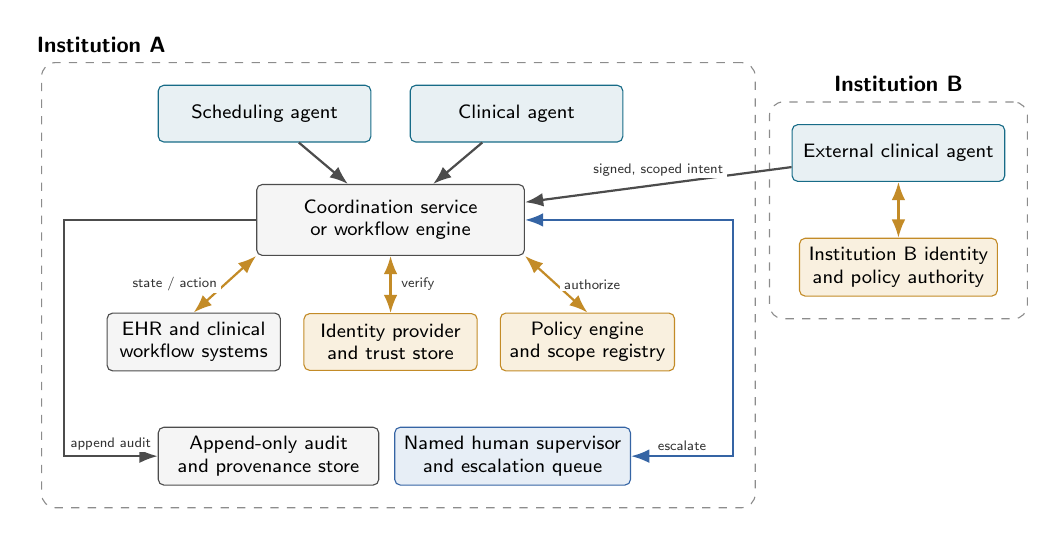
\begin{tikzpicture}[
  font=\sffamily\scriptsize,
  >=Latex,
  agent/.style={draw=circteal, fill=circteal!10, rounded corners=2pt,
    minimum width=2.7cm, minimum height=0.72cm, align=center},
  service/.style={draw=black!70, fill=black!4, rounded corners=2pt,
    minimum width=2.2cm, minimum height=0.72cm, align=center},
  control/.style={draw=circgold!90!black, fill=circgold!15, rounded corners=2pt,
    minimum width=2.2cm, minimum height=0.72cm, align=center},
  human/.style={draw=circblue!90!black, fill=circblue!12, rounded corners=2pt,
    minimum width=2.8cm, minimum height=0.72cm, align=center},
  boundary/.style={draw=black!45, dashed, rounded corners=5pt, inner sep=8pt},
  flow/.style={->, thick, draw=black!70},
  check/.style={<->, thick, draw=circgold!90!black},
  escalation/.style={<->, thick, draw=circblue!90!black},
  edgelabel/.style={fill=white, inner xsep=1.5pt, inner ysep=0.8pt,
    font=\sffamily\tiny, text=black!80}
]
  \node[agent] (agent1) at (-4.7,2.0) {Scheduling agent};
  \node[agent] (agent2) at (-1.5,2.0) {Clinical agent};
  \node[service, minimum width=3.4cm, minimum height=0.9cm] (coord) at (-3.1,0.65)
    {Coordination service\\or workflow engine};
  \node[service] (ehr) at (-5.6,-0.9) {EHR and clinical\\workflow systems};
  \node[control] (identity) at (-3.1,-0.9) {Identity provider\\and trust store};
  \node[control] (policy) at (-0.6,-0.9) {Policy engine\\and scope registry};
  \node[service, minimum width=2.8cm] (audit) at (-4.65,-2.35)
    {Append-only audit\\and provenance store};
  \node[human] (supervisor) at (-1.55,-2.35) {Named human supervisor\\and escalation queue};

  \node[agent] (external) at (3.35,1.5) {External clinical agent};
  \node[control] (externaltrust) at (3.35,0.05) {Institution B identity\\and policy authority};

  \coordinate (auditlane) at (-7.25,0.65);
  \coordinate (auditturn) at (-7.25,-2.35);
  \coordinate (escalationlane) at (1.25,0.65);
  \coordinate (escalationturn) at (1.25,-2.35);

  \draw[flow] (agent1) -- (coord);
  \draw[flow] (agent2) -- (coord);
  \draw[flow] (external) -- node[midway, above=2pt, edgelabel]
    {signed, scoped intent} (coord);
  \draw[check] (coord.south west) -- node[midway, left=1pt, edgelabel]
    {state / action} (ehr.north);
  \draw[check] (coord.south) -- node[midway, right=2pt, edgelabel] {verify} (identity.north);
  \draw[check] (coord.south east) -- node[midway, right=1pt, edgelabel]
    {authorize} (policy.north);
  \draw[flow] (coord.west) -- (auditlane) -- (auditturn)
    -- node[midway, above=1pt, edgelabel] {append audit} (audit.west);
  \draw[escalation] (coord.east) -- (escalationlane) -- (escalationturn)
    -- node[midway, above=1pt, edgelabel] {escalate} (supervisor.east);
  \draw[check] (external) -- (externaltrust);

  \begin{scope}[on background layer]
    \node[boundary,
      fit=(agent1)(agent2)(coord)(ehr)(identity)(policy)(audit)(supervisor)
          (auditlane)(auditturn)(escalationlane)(escalationturn),
      label={[font=\sffamily\bfseries\footnotesize]above left:Institution A}] {};
    \node[boundary, fit=(external)(externaltrust),
      label={[font=\sffamily\bfseries\footnotesize]above:Institution B}] {};
  \end{scope}
\end{tikzpicture}}
\caption{One possible implementation of CIRC governance levers. Identity, authorization, clinical
state, audit, and human escalation remain institutionally governed even when an external agent uses a
shared coordination message. The coordination service may be replaced by an EHR-native workflow or
another architecture that provides equivalent controls and evidence.}
\label{fig:architecture}
\end{figure}

\subsection{Implementation patterns and trade-offs}

The same governance lever can be realized through different architectures
(Table~\ref{tab:architectures}). The appropriate choice depends on institutional boundaries,
workflow stability, latency, reversibility, and the consequences of coordinator failure.

\begin{table}[htbp]
\centering
\caption{Alternative architectures for implementing CIRC governance levers.}
\label{tab:architectures}
\footnotesize
\begin{tabularx}{\linewidth}{B{0.19\linewidth}YY}
\toprule
Pattern & Principal strengths & Limitations and role of shared conventions \\
\midrule
Central workflow orchestrator & One authority for sequencing, retries, compensation, and human
tasks; clear operational ownership. & Can become a bottleneck or single failure domain; cross-vendor
inputs still need stable identity, intent, state, and outcome semantics. \\
EHR-native workflow control & Close to orders, patient context, existing permissions, and clinician
work queues. & May be vendor- or institution-specific and difficult to extend across external agents
or non-EHR systems. \\
Policy engine and identity layer & Centralized authorization, revocation, separation of duties, and
consistent policy decisions. & Does not by itself coordinate task state, clinical prerequisites,
resource contention, or human response. \\
Supervisory agent & Can synthesize context and detect conflicts without requiring every peer to
communicate directly. & Introduces another model failure surface; requires bounded authority,
independent monitoring, and deterministic enforcement for consequential actions. \\
Distributed agent protocol & Supports cross-vendor discovery, delegation, and task exchange without
one workflow owner. & Increases consistency, trust, conflict-resolution, and outage-recovery demands;
clinical profiles are needed above the transport. \\
Human-led coordination & Uses existing professional accountability and adapts to unusual cases. &
Limited by latency, workload, alert burden, and diffusion of responsibility; agent escalations still
need named recipients and closure rules. \\
\bottomrule
\end{tabularx}
\end{table}

CIRC asks whether the chosen architecture provides each needed control and evidence trail. A FHIR
implementation guide, A2A extension, or local orchestration policy may satisfy the contract; a new
primitive is warranted only when existing representations or conformance cannot.

\section{Failure model and degraded operation}

A coordination layer is itself safety-critical infrastructure and can create common-mode failure.
Systems-theoretic safety work likewise treats hazards as failures of interactions and control rather
than only failures of individual components.\cite{leveson2004new} CIRC therefore assumes that agents,
credentials, messages, state stores, dependency models,
coordinators, and human response processes can each fail or be compromised. It does not assume that
failures are independent or benign. The framework does not prescribe a universal identity issuer or
consistency algorithm; it requires each deployment to declare its trust anchors, revocation mechanism,
state guarantees, and degraded behavior. This follows a zero-trust posture in which access is
evaluated for the requesting subject, resource, and context rather than inferred from network
location.\cite{rose2020zerotrust}

Table~\ref{tab:failure-model} states the principal failure surfaces. The controls are illustrative:
their adequacy depends on clinical consequences, timing, reversibility, and organizational boundaries.
Classical state-machine replication can improve availability and consistency, for example, but does
not make an incorrect dependency model clinically correct.\cite{schneider1990statemachine}

\begin{table}[htbp]
\centering
\caption{Failure model for the clinical-agent coordination layer.}
\label{tab:failure-model}
\footnotesize
\begin{tabularx}{\linewidth}{B{0.19\linewidth}YY}
\toprule
Failure surface & Illustrative failures & Required containment behavior \\
\midrule
Identity and trust & Compromised agent; false scope declaration; credential theft; stale or
unrevoked credential; untrusted external issuer. & Verify issuer, audience, version, delegation, and
revocation at decision time; reject or quarantine the actor; preserve evidence for incident review. \\
State and messaging & Stale patient state; loss, duplication, reordering, or replay; conflicting
versions; delayed acknowledgement; network partition. & Bind actions to state versions; use
idempotency and replay protection; expose uncertainty; prevent irreversible execution on unresolved
state. \\
Dependency and workflow & Missing or incorrect prerequisite; cyclic dependency; deadlock or
livelock; unbounded retry; partial cancellation or compensation. & Validate graphs, bound retries,
detect cycles, propagate cancellation, and freeze the affected pathway when consistency cannot be
restored. \\
Arbitration and resource signals & Incorrect priority; manipulated or stale capacity; starvation;
correlated demand; denial of service. & Authenticate and timestamp aggregate signals, enforce rate
and fairness policies, detect concentration, and transfer allocation to a designated fallback. \\
Coordination service & Outage, corrupted state, faulty arbitration, software update failure, or loss
of quorum. & Use health checks and redundancy appropriate to risk; expose degraded status; restore
from auditable checkpoints; avoid silent continuation under unknown control state. \\
Human control path & Alert not delivered or acknowledged; wrong recipient; alert overload;
automation bias; conflicting overrides; diffusion of responsibility. & Require named ownership,
deadline and acknowledgement, fallback escalation, override authority, workload monitoring, and
documented closure. \\
\bottomrule
\end{tabularx}
\end{table}

Safe mode should be defined by action class rather than by one universal ``fail closed'' rule.
Read-only retrieval or analysis may continue during partial outage only when data freshness and
missing coordination context are visible to the user. Reversible administrative actions may be
queued, deduplicated, or released after explicit confirmation. Actions that change treatment, orders,
medication, disposition, or other consequential clinical state should generally be held when identity,
scope, prerequisite, or shared-state checks are unavailable. Emergency exceptions require a
predefined institutional pathway; the coordination layer should not invent one at runtime. In every
case, the system should identify which guarantees remain active, return control to a named role, and
record how normal operation was restored.

Cross-organizational identity requires federation rather than one global CIRC authority. Each
institution can issue or recognize credentials under its own policy, while bilateral or network trust
agreements define accepted issuers, assurance levels, claims, and revocation expectations. A valid
identity establishes attribution, not clinical authority: authorization remains specific to the
patient, action, setting, time, and delegated purpose.

\section{Operational human oversight}

``Human review'' is not a control unless it changes who is responsible for what happens next. Health
IT safety is sociotechnical: performance depends on people, tasks, technology, organizations, and the
environment in which they interact.\cite{sittig2010sociotechnical,carayon2006seips} Automation can
also redistribute attention and authority rather than simply reduce workload.\cite{parasuraman2000automation}
CIRC therefore treats oversight as an operational contract, not an endpoint label.

Every escalation should specify: (1) the accountable role and current assignee; (2) the triggering
condition and supporting evidence; (3) the decision or action requested; (4) urgency and a response
deadline; (5) whether the proposed action is blocked, queued, or continuing; (6) the fallback recipient
and behavior after non-response; and (7) the event that closes the escalation. Assignment, delivery,
acknowledgement, decision, override, and closure should be distinct auditable states.

Institutions must also define governance outside the immediate alert. A designated body should
approve agent scopes and material changes; operational owners should be able to pause an agent;
credential and policy administrators should revoke access; and a clinical authority should resolve
conflicting recommendations. Separation of duties is important when one vendor supplies both the
acting agent and the supervisory component. Escalation policies should suppress duplicates, group
related concerns, set alert budgets, and monitor acknowledgement and override patterns so that adding
a coordination layer does not simply add another source of alert fatigue.

Useful oversight measures include time to assignment, acknowledgement, and decision; fraction of
escalations with no response by deadline; fallback activation; duplicate-alert rate; override and
reversal rate; unresolved workload per accountable role; and the fraction of consequential actions
executed without documented closure. These measures evaluate the response process rather than merely
counting alerts.

\section{Regulatory and institutional positioning}

\begin{table}[!t]
\centering
\caption{Regulatory obligations, CIRC operational evidence, and unresolved boundaries.}
\label{tab:regulatory-boundary}
\footnotesize
\begin{tabularx}{\linewidth}{B{0.17\linewidth}p{0.23\linewidth}YY}
\toprule
Context & Existing obligation or decision & CIRC operationalization & Not resolved by CIRC \\
\midrule
U.S. function classification & Intended use and statutory criteria determine whether a CDS function
is a device. & Inventory each function, user, action, autonomy, and responsible organization. & Legal
status, intended-use claims, and applicable submission pathway. \\
FDA device lifecycle & Premarket evidence and, when authorized, a PCCP govern specified AI-enabled
device changes. & Bind versions and modifications to validation, impact assessment, monitoring, and
rollback evidence. & Safety or effectiveness, authorization of a change, and reporting thresholds. \\
EU high-risk provider duties & Risk management, logs, oversight, robustness, quality management, and
post-market monitoring (Arts. 9, 12, 14, 15, 17, 72). & Link identity, policy, dependency, escalation,
safe-mode, and recovery records across agents. & High-risk classification, conformity assessment,
fundamental-rights analysis, and provider liability. \\
EU deployer and institutional duties & Human oversight, log retention, monitoring, and incident action
apply according to role and context (Art. 26). & Name local owners, deadlines, fallback, pause
authority, closure, and affected workflows. & Professional responsibility, staffing adequacy, local
law, and allocation of responsibility across vendors. \\
\bottomrule
\end{tabularx}
\end{table}

Regulatory status attaches to a software function, its intended use, users, claims, and deployment
context---not to the labels ``agent'' or ``CIRC'' and not to a centralized or distributed topology.
In the United States, FDA guidance distinguishes clinical decision support functions that satisfy the
statutory non-device criteria from software functions that remain devices.\cite{fda2026cds} A
multi-agent deployment may contain administrative functions, non-device decision support, and device
software functions at the same time. Each function therefore requires its own assessment, including
whether combining it with autonomous execution or other agents changes its intended use or risk.

For an AI-enabled device software function, an authorized predetermined change control plan can
describe specified future modifications, the method for developing, validating, and implementing
them, and the associated impact assessment.\cite{fda2025pccp} CIRC records such as stable versions,
delegation, policy decisions, dependency checks, reversals, and post-deployment events could support
that lifecycle evidence. They do not establish safety or effectiveness, expand the authorized
intended use, or make an out-of-plan modification permissible.

The European Union AI Act likewise bases obligations on intended purpose, statutory role, and
classification. For systems classified as high-risk, Articles 9, 12, 14, 15, 17, and 72 address risk
management, record keeping, human oversight, accuracy, robustness and cybersecurity, quality
management, and post-market monitoring; Article 26 defines deployer duties.\cite{eu2024aiact} CIRC
levers overlap with several of these operational concerns, but implementing a lever is not itself a
demonstration of conformity. Privacy, cybersecurity, medical-device, professional-practice, and
health-system obligations also remain independently applicable.

The residual coordination gap is therefore operational rather than a claim that regulation is absent.
High-level duties do not by themselves specify cross-agent state versions, dependency semantics,
timeout and fallback behavior, or common evidence across vendor boundaries. CIRC offers a vocabulary
for those interfaces while leaving classification, conformity, liability, and enforcement to the
applicable authorities and institutions.

Before release, a deployment dossier should therefore map every consequential action to the function
that proposes and executes it, its intended use and autonomy, the responsible legal and operational
actors, applicable authorization, validation evidence, dependencies, affected populations, and
fallback behavior. Changes to a model or agent version, permitted action, dependency, trust boundary,
patient population, resource policy, or human fallback should trigger a recorded impact assessment
proportional to the risk. This is an institutional change-control rule, not a claim that every change
requires a new regulatory submission.

\section{From risk taxonomy to evaluation}

The taxonomy separates three questions that were conflated in the submitted simulations. First, can
a risk be observed? Candidate measures include attribution completeness, stale-state reads,
unresolved dependencies, duplicated or conflicting actions, retry amplification, queue concentration,
safe-mode activation, and unowned or overdue escalations. Second, can a control detect or contain the risk without blocking valid work?
Matched stress tests should report both fault containment and preservation of unaffected workflows.
Third, does the control improve clinical or operational outcomes? That question requires prospective
evaluation and cannot be inferred from a deterministic demonstration.

Trace-based benchmarks such as CliniCARE provide a concrete template for the first question. They log
retrieval, computation, policy access, citations, and reports, allowing process defects to be separated
from final-answer errors without inspecting private reasoning. Extending this approach to interaction
risks would require linked traces from multiple agents acting on shared state, together with
prespecified fault models, applicable denominators, baselines, repeated runs, uncertainty estimates,
and failure cases. Population-level resource tests would additionally need realistic arrival
processes, capacity constraints, and human response models.

Accordingly, this Perspective does not present the removed toy simulations as evidence of control
effectiveness. Instead, it proposes a staged evaluation agenda: trace-based assessment of agent-local
risks; matched multi-agent replay for interaction and workflow risks; system stress testing for shared
resources and common-mode failure; prospective shadow deployment; and monitored clinical use where
regulatory and institutional requirements permit.

\section{Limitations and future directions}

CIRC is a conceptual and non-exhaustive framework. It does not specify a complete technical
implementation, establish the necessity or sufficiency of any lever, certify deployment readiness, or
demonstrate clinical benefit. The taxonomy will require extension as clinical agents acquire new
capabilities and as evidence emerges from real workflows. Its categories also overlap: a stale-state
error, for example, can reflect an agent-local retrieval failure, an interaction failure, and an
institutional monitoring failure.

CliniCARE illustrates trace-observable agent-local risks, but it is a retrospective single-agent audit
benchmark rather than a test of multi-agent coordination. Its findings cannot support claims about
cross-vendor messaging, shared-resource control, human response, or prevented patient harm. Likewise,
population-level clinical prediction is outside the scope of a coordination framework and must be
developed and validated as a separate clinical model.

The threat model and oversight contract identify requirements but do not establish that any proposed
implementation will satisfy them. Choices about trusted issuers, consistency, emergency exceptions,
response deadlines, and safe-mode behavior remain institution- and action-specific. Governance
questions also include liability, local configuration, alert burden, and equitable access. The
regulatory discussion above is descriptive rather than legal guidance; applicability depends on the
specific function, intended use, jurisdiction, and organizational role. Future work should compare
protocol, orchestration, policy-engine, EHR-native, and human-led implementations against common
risk-specific endpoints.

\section{Conclusion}

Multi-agent clinical safety cannot be inferred from individual-agent performance alone. The relevant
risks span local investigations, interactions across shared workflows, and the institutions that
authorize, monitor, and respond to autonomous action. CIRC offers a starting taxonomy for those risks
and a set of independent governance levers that can be implemented through different technical
architectures.

The framework's value should be judged by whether it makes requirements and evidence more precise,
not by treating its categories as a maturity ladder or its controls as established safety invariants.
Existing trace-based benchmarks show how some agent-local risks can be measured. The next challenge is
to build equally inspectable evaluations for shared state, dependencies, resource competition,
degraded operation, and human response before autonomous clinical agents operate at scale.

\section*{Acknowledgments}
The authors received no specific funding for this work.

\section*{Author contributions}
B.C.X. contributed to conceptualization, methodology, investigation, visualization, drafting, and
review and editing. A.C. contributed to conceptualization, methodology, and review and editing.
A.J.R. contributed to conceptualization, supervision, and review and editing.

\section*{Competing interests}
The authors declare no competing interests.

\bibliographystyle{unsrtnat}
\bibliography{references}

\end{document}